\chapter{Running a Program}
\label{ch:running}

A program is loaded in the Files browser, checked on the Program page, and started from the
panel. LiNC never starts a program by itself and never starts one when you load it.

\section{Loading a program}

\begin{itemize}
  \item Press \keycap{F6} for Program, then \keycap{F6} again for Files. On any other page,
        \chordtwo{Ctrl}{O} opens Files directly.
  \item The right-hand pane lists the program directory. It comes from the controller's
        \texttt{PROGRAM\_PREFIX}; there is no second copy of that path in the interface.
  \item The left-hand pane shows removable media. \keycap{Enter} on a file there copies it
        into the program directory.
  \item \keycap{Enter} on a program in the right-hand pane loads it.
\end{itemize}

Loading always does the same four things: it closes Files, switches to Program in the
\sbtn{SPLIT} layout, fits the toolpath and highlights line 1. It does not start anything, and
it does not change the panel's mode.

\begin{cautionbox}
  Only files inside the program directory are loaded. The controller will not accept a path
  outside it, and LiNC does not offer one.
\end{cautionbox}

\shot{img/ui/files.png}{The Files browser: removable media on the left, the program directory on
the right. Every action is a key; there is no button row.}{fig:files}

\section{Checking the program}

\begin{figure}[H]
  \centering
  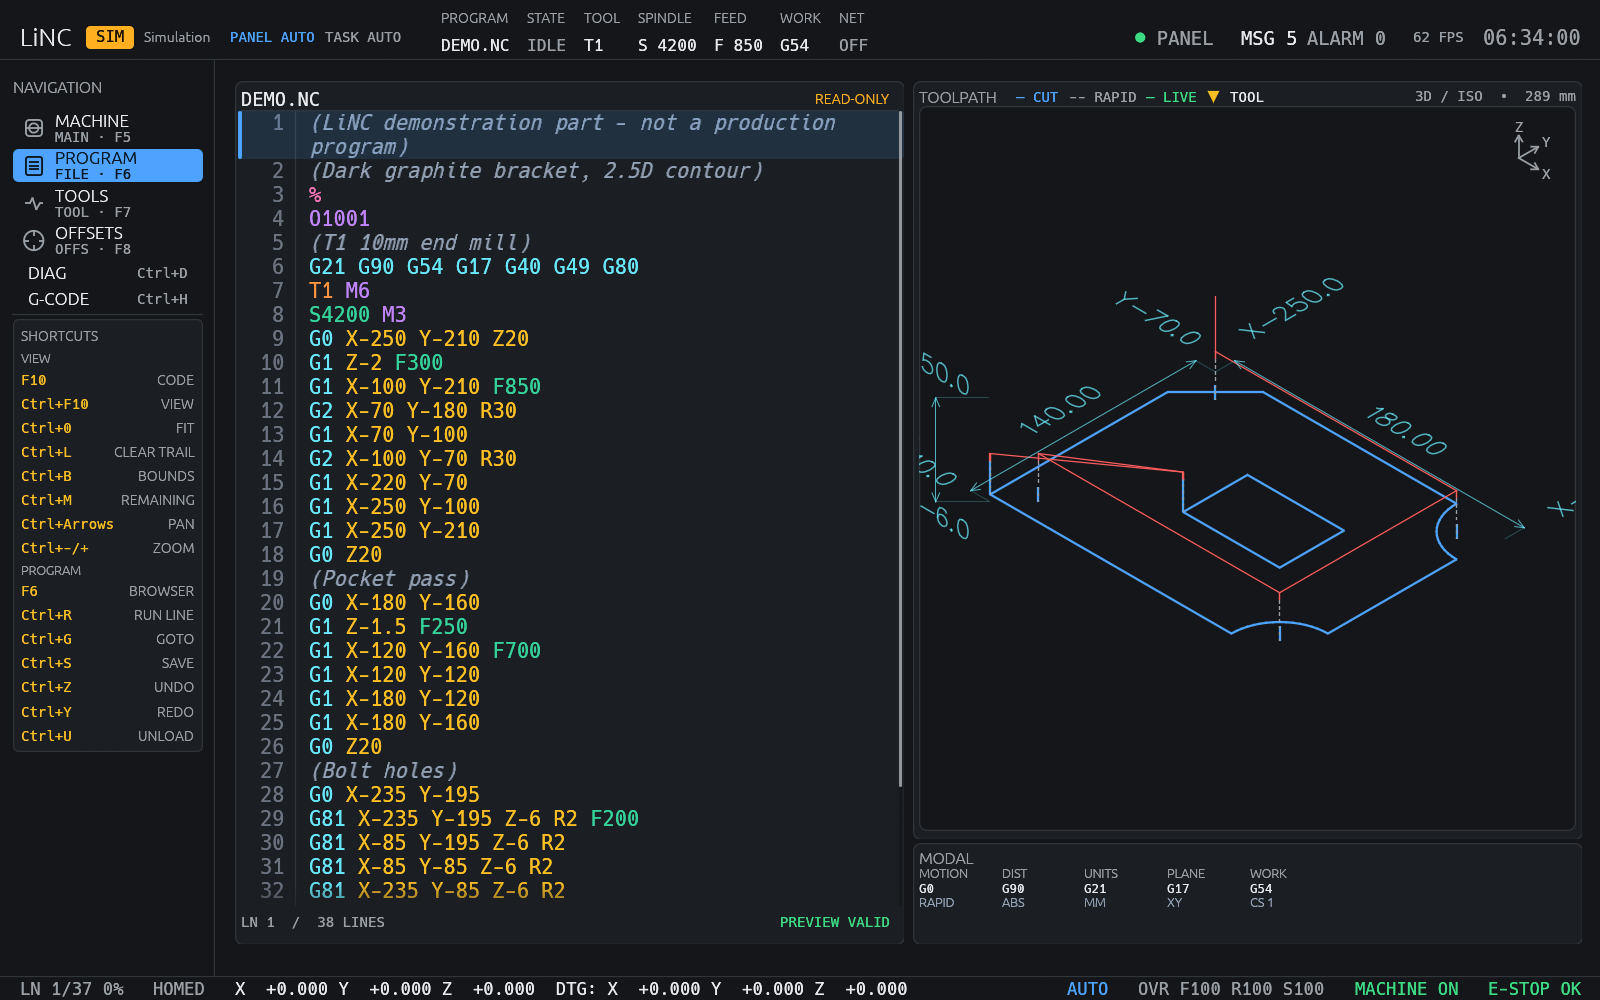
\includegraphics[width=\textwidth]{img/ui/program.png}
  \caption{The Program page in SPLIT: editor or monitor on the left, toolpath on the right,
           modal codes under it.}
  \label{fig:program-page}
\end{figure}

The Program page is the checking surface, and the Machine page is the running surface.

\begin{itemize}
  \item \textbf{The path tells you what the machine will do.} The loaded program is drawn in
        program colours with dotted rapids. Anything outside the machine's travel envelope is
        drawn solid red, split at the exact crossing, so a program that would crash is
        visible before it runs.
  \item \textbf{RED means outside the machine.} It is not a style accent and it is not a
        warning about the toolpath's shape.
  \item \textbf{The preview validates.} A parse error keeps the last valid drawing and marks
        the offending line; it never draws a guess.
  \item \textbf{The modal pane} shows the active units, plane, motion mode, work system and
        compensation, read from the controller as the program runs.
  \item \textbf{The G-code help} answers questions offline: \chordtwo{Ctrl}{H}.
\end{itemize}

The Machine page carries the same toolpath plus the program card: the listing with the
executing line, the modal band, the progress bar and a status word. That word reads
\state{RUNNING}, \state{PAUSED} or \state{STOP}. It is a readout. There is no stop button on
the screen.

\section{Starting the program: cycle start}

The panel's \pbtn{CYCLE START} starts the loaded program. The controller gates it, and the
usual conditions are:

\begin{itemize}
  \item machine power on, no emergency stop,
  \item every axis homed,
  \item the interpreter idle: not running, not waiting for a tool change,
  \item the panel's mode selector in \textbf{AUTO},
  \item panel data current, program protect irrelevant to running but relevant to editing.
\end{itemize}

LiNC does not issue cycle start. It shows the line and the progress, and it shows the
controller's own error in the messages when a start is refused.

\section{Starting at a line: RUN FROM LINE}

\chordtwo{Ctrl}{R} on the Program page starts the loaded program at the selected line.
A line number is the one program-start input the panel cannot supply, so this is the only
program start the interface issues.

\begin{itemize}
  \item It runs only when a program is loaded, the interpreter is idle, the machine is on, no
        emergency stop is latched, every axis is homed, the panel data is current and the
        selector is in AUTO.
  \item A confirmation names the line and its block and states that the lines before it are
        skipped: work and tool offsets, feed, spindle and coolant are not restored, and
        motion starts from the current position.
  \item When a condition blocks it, the reason is shown as a message. The key does not go
        quiet.
\end{itemize}

\section{Finding a line: GO TO LINE}

\chordtwo{Ctrl}{G} asks for a line number and moves the program view there. The editor,
the path highlight and the Machine page's program card follow it. While the program runs the
view normally follows the executing line; a line you chose with \chordtwo{Ctrl}{G} or
the arrow keys is kept until the next run starts.

\section{While the program runs}

\begin{itemize}
  \item The executing line is marked in the listing with a bar and a tinted row, and the view
        scrolls to keep it visible.
  \item The bottom bar shows \state{LN 12/340 34\%}: the executing line, the line count and
        the progress.
  \item The Machine page's toolpath draws the live tool trail in its own colour, separate
        from the program path. \chordtwo{Ctrl}{L} clears the trail without touching
        the program.
  \item \chordtwo{Ctrl}{M} switches to REMAINING: the trail disappears and every block
        already cut is eaten out of the program path, so the card shows only what is left.
  \item Feed hold, single block, block delete, optional stop and cycle stop are panel keys.
        They are wired to the controller, not to LiNC.
\end{itemize}

\begin{notebox}
  The editor is read-only while a program runs. Clicking into the listing selects a line for
  the view; it does not edit the running program, because the controller runs the copy it
  opened, not the buffer.
\end{notebox}

\section{Stopping and resetting}

\begin{itemize}
  \item \pbtn{CYCLE STOP} on the panel stops the program and stops motion.
  \item \keycap{Esc} resets: it aborts the program at the controller and rewinds the
        interpreter. The program stays loaded and can be started again.
  \item A paused program is resumed by cycle start, not by RUN FROM LINE: the controller
        refuses a run-from-line on a paused program rather than resuming it at the wrong
        place.
\end{itemize}

\section{Unloading the program}
\label{sec:unload}

\chordtwo{Ctrl}{U} on the Program page unloads the program and releases the external
network link.

What it does, in order:

\begin{enumerate}
  \item It refuses to run while the program is running (\state{PROGRAM RUNNING — STOP FIRST}),
        with unsaved changes (\state{UNSAVED CHANGES — SAVE OR REVERT FIRST}) or with nothing
        loaded (\state{NO PROGRAM LOADED}).
  \item It sends the controller's program close, then resets the interpreter.
  \item It re-reads the program name from the controller. If the controller still names a
        program, the unload fails loudly with \state{the controller kept the program after
        close} instead of pretending to succeed.
  \item It shows \state{UNLOAD REQUESTED — WATCH NET}. The \state{NET} field returns to
        \state{UP} within a few seconds, once the radio is associated and a default route
        exists.
\end{enumerate}

Unloading also clears the editor and the toolpath on the Program page when the controller
reports that no program is loaded.

\begin{tipbox}
  If the network does not come back, look at the \state{NET} field, not at the WiFi menu.
  \state{?} means the state is unknown; \state{UP} means the link is back. The interface
  writes the interlock's \halpin{net-safe} output and the machine HAL does the rest.
\end{tipbox}

\section{Program changed on disk}

If the file on disk changes while it is open in the buffer, Program shows the banner
\state{PROGRAM CHANGED EXTERNALLY — unsaved buffer preserved. Save will use the current
revision.} The buffer does not reload itself and does not lose your edits. Decide: save over
the new file, or discard and load again.
